% Options for packages loaded elsewhere
\PassOptionsToPackage{unicode}{hyperref}
\PassOptionsToPackage{hyphens}{url}
%
\documentclass[
]{article}
\usepackage{amsmath,amssymb}
\usepackage{lmodern}
\usepackage{ifxetex,ifluatex}
\ifnum 0\ifxetex 1\fi\ifluatex 1\fi=0 % if pdftex
  \usepackage[T1]{fontenc}
  \usepackage[utf8]{inputenc}
  \usepackage{textcomp} % provide euro and other symbols
\else % if luatex or xetex
  \usepackage{unicode-math}
  \defaultfontfeatures{Scale=MatchLowercase}
  \defaultfontfeatures[\rmfamily]{Ligatures=TeX,Scale=1}
\fi
% Use upquote if available, for straight quotes in verbatim environments
\IfFileExists{upquote.sty}{\usepackage{upquote}}{}
\IfFileExists{microtype.sty}{% use microtype if available
  \usepackage[]{microtype}
  \UseMicrotypeSet[protrusion]{basicmath} % disable protrusion for tt fonts
}{}
\makeatletter
\@ifundefined{KOMAClassName}{% if non-KOMA class
  \IfFileExists{parskip.sty}{%
    \usepackage{parskip}
  }{% else
    \setlength{\parindent}{0pt}
    \setlength{\parskip}{6pt plus 2pt minus 1pt}}
}{% if KOMA class
  \KOMAoptions{parskip=half}}
\makeatother
\usepackage{xcolor}
\IfFileExists{xurl.sty}{\usepackage{xurl}}{} % add URL line breaks if available
\IfFileExists{bookmark.sty}{\usepackage{bookmark}}{\usepackage{hyperref}}
\hypersetup{
  pdftitle={R Notebook},
  hidelinks,
  pdfcreator={LaTeX via pandoc}}
\urlstyle{same} % disable monospaced font for URLs
\usepackage[margin=1in]{geometry}
\usepackage{color}
\usepackage{fancyvrb}
\newcommand{\VerbBar}{|}
\newcommand{\VERB}{\Verb[commandchars=\\\{\}]}
\DefineVerbatimEnvironment{Highlighting}{Verbatim}{commandchars=\\\{\}}
% Add ',fontsize=\small' for more characters per line
\usepackage{framed}
\definecolor{shadecolor}{RGB}{248,248,248}
\newenvironment{Shaded}{\begin{snugshade}}{\end{snugshade}}
\newcommand{\AlertTok}[1]{\textcolor[rgb]{0.94,0.16,0.16}{#1}}
\newcommand{\AnnotationTok}[1]{\textcolor[rgb]{0.56,0.35,0.01}{\textbf{\textit{#1}}}}
\newcommand{\AttributeTok}[1]{\textcolor[rgb]{0.77,0.63,0.00}{#1}}
\newcommand{\BaseNTok}[1]{\textcolor[rgb]{0.00,0.00,0.81}{#1}}
\newcommand{\BuiltInTok}[1]{#1}
\newcommand{\CharTok}[1]{\textcolor[rgb]{0.31,0.60,0.02}{#1}}
\newcommand{\CommentTok}[1]{\textcolor[rgb]{0.56,0.35,0.01}{\textit{#1}}}
\newcommand{\CommentVarTok}[1]{\textcolor[rgb]{0.56,0.35,0.01}{\textbf{\textit{#1}}}}
\newcommand{\ConstantTok}[1]{\textcolor[rgb]{0.00,0.00,0.00}{#1}}
\newcommand{\ControlFlowTok}[1]{\textcolor[rgb]{0.13,0.29,0.53}{\textbf{#1}}}
\newcommand{\DataTypeTok}[1]{\textcolor[rgb]{0.13,0.29,0.53}{#1}}
\newcommand{\DecValTok}[1]{\textcolor[rgb]{0.00,0.00,0.81}{#1}}
\newcommand{\DocumentationTok}[1]{\textcolor[rgb]{0.56,0.35,0.01}{\textbf{\textit{#1}}}}
\newcommand{\ErrorTok}[1]{\textcolor[rgb]{0.64,0.00,0.00}{\textbf{#1}}}
\newcommand{\ExtensionTok}[1]{#1}
\newcommand{\FloatTok}[1]{\textcolor[rgb]{0.00,0.00,0.81}{#1}}
\newcommand{\FunctionTok}[1]{\textcolor[rgb]{0.00,0.00,0.00}{#1}}
\newcommand{\ImportTok}[1]{#1}
\newcommand{\InformationTok}[1]{\textcolor[rgb]{0.56,0.35,0.01}{\textbf{\textit{#1}}}}
\newcommand{\KeywordTok}[1]{\textcolor[rgb]{0.13,0.29,0.53}{\textbf{#1}}}
\newcommand{\NormalTok}[1]{#1}
\newcommand{\OperatorTok}[1]{\textcolor[rgb]{0.81,0.36,0.00}{\textbf{#1}}}
\newcommand{\OtherTok}[1]{\textcolor[rgb]{0.56,0.35,0.01}{#1}}
\newcommand{\PreprocessorTok}[1]{\textcolor[rgb]{0.56,0.35,0.01}{\textit{#1}}}
\newcommand{\RegionMarkerTok}[1]{#1}
\newcommand{\SpecialCharTok}[1]{\textcolor[rgb]{0.00,0.00,0.00}{#1}}
\newcommand{\SpecialStringTok}[1]{\textcolor[rgb]{0.31,0.60,0.02}{#1}}
\newcommand{\StringTok}[1]{\textcolor[rgb]{0.31,0.60,0.02}{#1}}
\newcommand{\VariableTok}[1]{\textcolor[rgb]{0.00,0.00,0.00}{#1}}
\newcommand{\VerbatimStringTok}[1]{\textcolor[rgb]{0.31,0.60,0.02}{#1}}
\newcommand{\WarningTok}[1]{\textcolor[rgb]{0.56,0.35,0.01}{\textbf{\textit{#1}}}}
\usepackage{longtable,booktabs,array}
\usepackage{calc} % for calculating minipage widths
% Correct order of tables after \paragraph or \subparagraph
\usepackage{etoolbox}
\makeatletter
\patchcmd\longtable{\par}{\if@noskipsec\mbox{}\fi\par}{}{}
\makeatother
% Allow footnotes in longtable head/foot
\IfFileExists{footnotehyper.sty}{\usepackage{footnotehyper}}{\usepackage{footnote}}
\makesavenoteenv{longtable}
\usepackage{graphicx}
\makeatletter
\def\maxwidth{\ifdim\Gin@nat@width>\linewidth\linewidth\else\Gin@nat@width\fi}
\def\maxheight{\ifdim\Gin@nat@height>\textheight\textheight\else\Gin@nat@height\fi}
\makeatother
% Scale images if necessary, so that they will not overflow the page
% margins by default, and it is still possible to overwrite the defaults
% using explicit options in \includegraphics[width, height, ...]{}
\setkeys{Gin}{width=\maxwidth,height=\maxheight,keepaspectratio}
% Set default figure placement to htbp
\makeatletter
\def\fps@figure{htbp}
\makeatother
\setlength{\emergencystretch}{3em} % prevent overfull lines
\providecommand{\tightlist}{%
  \setlength{\itemsep}{0pt}\setlength{\parskip}{0pt}}
\setcounter{secnumdepth}{-\maxdimen} % remove section numbering
\ifluatex
  \usepackage{selnolig}  % disable illegal ligatures
\fi

\title{R Notebook}
\author{}
\date{\vspace{-2.5em}}

\begin{document}
\maketitle

\begin{Shaded}
\begin{Highlighting}[]
\FunctionTok{library}\NormalTok{(knitr)}
\end{Highlighting}
\end{Shaded}

\begin{verbatim}
## Warning: package 'knitr' was built under R version 4.0.5
\end{verbatim}

\begin{Shaded}
\begin{Highlighting}[]
\NormalTok{usuarios }\OtherTok{=} \FunctionTok{read.table}\NormalTok{(}\StringTok{"usuarios5.csv"}\NormalTok{, }\AttributeTok{header =} \ConstantTok{TRUE}\NormalTok{, }\AttributeTok{sep =} \StringTok{","}\NormalTok{)}
\NormalTok{recorridos }\OtherTok{=} \FunctionTok{read.table}\NormalTok{(}\StringTok{"recorridos5.csv"}\NormalTok{, }\AttributeTok{header =} \ConstantTok{TRUE}\NormalTok{, }\AttributeTok{sep =} \StringTok{","}\NormalTok{)}
\NormalTok{usuarios}\SpecialCharTok{$}\NormalTok{genero\_usuario }\OtherTok{=} \FunctionTok{as.factor}\NormalTok{(usuarios}\SpecialCharTok{$}\NormalTok{genero\_usuario)}
\NormalTok{usuarios\_recorridos }\OtherTok{=} \FunctionTok{merge}\NormalTok{(usuarios, recorridos)}

\FunctionTok{attach}\NormalTok{(recorridos)}

\NormalTok{dias }\OtherTok{=} \FunctionTok{factor}\NormalTok{(recorridos}\SpecialCharTok{$}\NormalTok{dia, }\AttributeTok{levels =} \FunctionTok{c}\NormalTok{(}\StringTok{"Domingo"}\NormalTok{, }\StringTok{"Lunes"}\NormalTok{, }\StringTok{"Martes"}\NormalTok{, }\StringTok{"Miércoles"}\NormalTok{, }\StringTok{"Jueves"}\NormalTok{, }\StringTok{"Viernes"}\NormalTok{, }\StringTok{"Sábado"}\NormalTok{))}
\NormalTok{usuarios\_recorridos}\SpecialCharTok{$}\NormalTok{dia }\OtherTok{=} \FunctionTok{factor}\NormalTok{(dias)}

\NormalTok{direcciones }\OtherTok{=} \FunctionTok{as.factor}\NormalTok{(}\FunctionTok{c}\NormalTok{(direccion\_estacion\_origen, direccion\_estacion\_destino))}

\NormalTok{vn }\OtherTok{=} \FunctionTok{sort}\NormalTok{(}\FunctionTok{table}\NormalTok{(direcciones), }\AttributeTok{decreasing =} \ConstantTok{TRUE}\NormalTok{)}
\NormalTok{vn2 }\OtherTok{=} \FunctionTok{sort}\NormalTok{(vn, }\AttributeTok{decreasing =} \ConstantTok{TRUE}\NormalTok{)[}\DecValTok{1}\SpecialCharTok{:}\DecValTok{10}\NormalTok{]}
\end{Highlighting}
\end{Shaded}

Top 10 estaciones

\begin{Shaded}
\begin{Highlighting}[]
\FunctionTok{par}\NormalTok{(}\AttributeTok{mar=}\FunctionTok{c}\NormalTok{(}\DecValTok{5}\NormalTok{,}\DecValTok{13}\NormalTok{,}\DecValTok{2}\NormalTok{,}\DecValTok{2}\NormalTok{))}
\FunctionTok{barplot}\NormalTok{(}\FunctionTok{sort}\NormalTok{(vn2, }\AttributeTok{decreasing =} \ConstantTok{FALSE}\NormalTok{), }\AttributeTok{las=}\DecValTok{1}\NormalTok{, }\AttributeTok{xlim =} \FunctionTok{c}\NormalTok{(}\DecValTok{0}\NormalTok{, }\DecValTok{40}\NormalTok{), }\AttributeTok{xlab =} \StringTok{"Usos"}\NormalTok{, }\AttributeTok{col =} \FunctionTok{rainbow}\NormalTok{(}\DecValTok{10}\NormalTok{), }\AttributeTok{horiz =} \ConstantTok{TRUE}\NormalTok{, }\AttributeTok{cex.names=}\FloatTok{0.7}\NormalTok{)}
\end{Highlighting}
\end{Shaded}

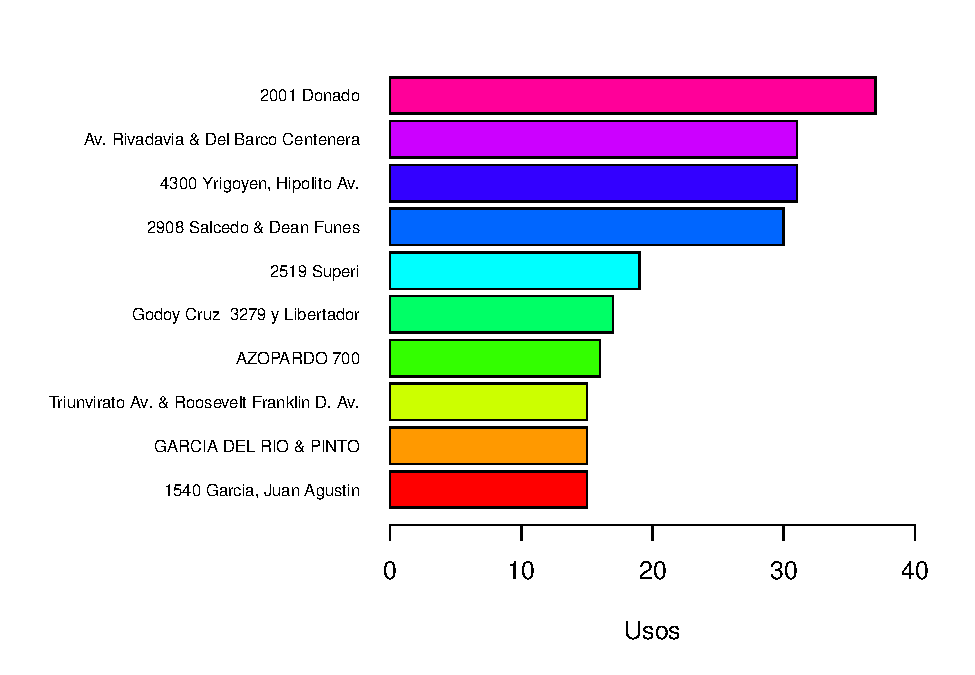
\includegraphics{notebook_files/figure-latex/unnamed-chunk-2-1.pdf} Uso
de Estaciones

\begin{Shaded}
\begin{Highlighting}[]
\FunctionTok{par}\NormalTok{(}\AttributeTok{mar=}\FunctionTok{c}\NormalTok{(}\DecValTok{4}\NormalTok{,}\DecValTok{4}\NormalTok{,}\DecValTok{4}\NormalTok{,}\DecValTok{2}\NormalTok{))}
\FunctionTok{plot}\NormalTok{(vn, }\AttributeTok{ylim =} \FunctionTok{c}\NormalTok{(}\DecValTok{0}\NormalTok{, }\DecValTok{40}\NormalTok{), }\AttributeTok{xaxt=}\StringTok{\textquotesingle{}n\textquotesingle{}}\NormalTok{, }\AttributeTok{xlab =} \StringTok{"Paradas"}\NormalTok{, }\AttributeTok{ylab =} \StringTok{"Usos"}\NormalTok{, }\AttributeTok{col =} \FunctionTok{rainbow}\NormalTok{(}\DecValTok{1200}\NormalTok{))}
\end{Highlighting}
\end{Shaded}

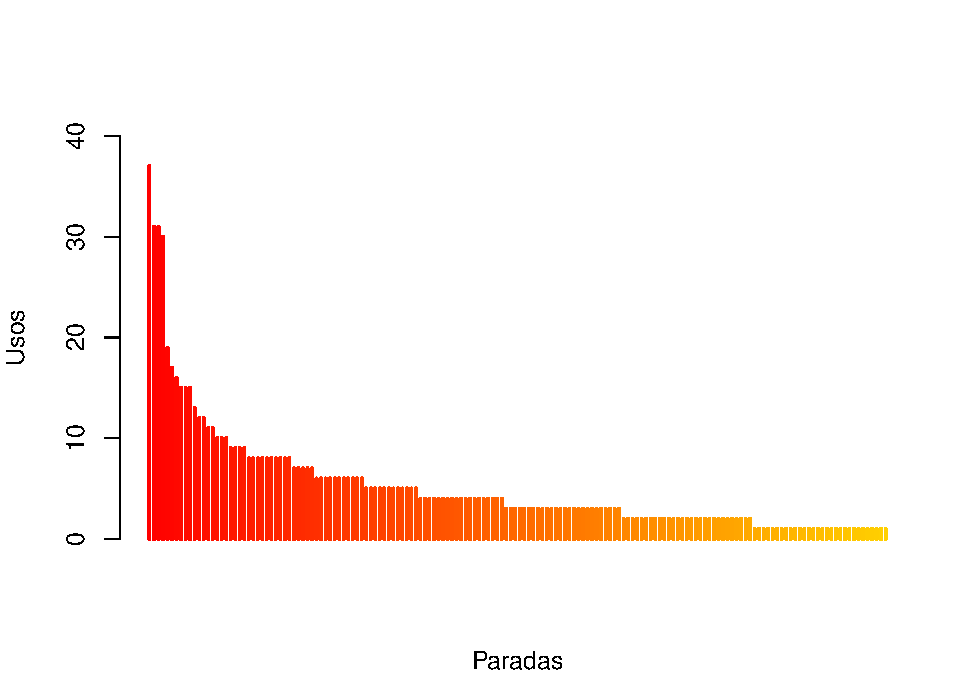
\includegraphics{notebook_files/figure-latex/unnamed-chunk-3-1.pdf}

Viajes cada Dia

\begin{Shaded}
\begin{Highlighting}[]
\NormalTok{viajes\_semana }\OtherTok{=} \FunctionTok{table}\NormalTok{(usuarios\_recorridos}\SpecialCharTok{$}\NormalTok{dia)}
\FunctionTok{barplot}\NormalTok{(viajes\_semana, }\AttributeTok{xlab =} \StringTok{"Dia"}\NormalTok{, }\AttributeTok{ylab =} \StringTok{"Viajes"}\NormalTok{, }\AttributeTok{names =} \FunctionTok{levels}\NormalTok{(dias), }\AttributeTok{col =} \FunctionTok{rainbow}\NormalTok{(}\DecValTok{7}\NormalTok{), }\AttributeTok{beside =} \ConstantTok{TRUE}\NormalTok{, }\AttributeTok{cex.names =} \FloatTok{0.9}\NormalTok{)}
\end{Highlighting}
\end{Shaded}

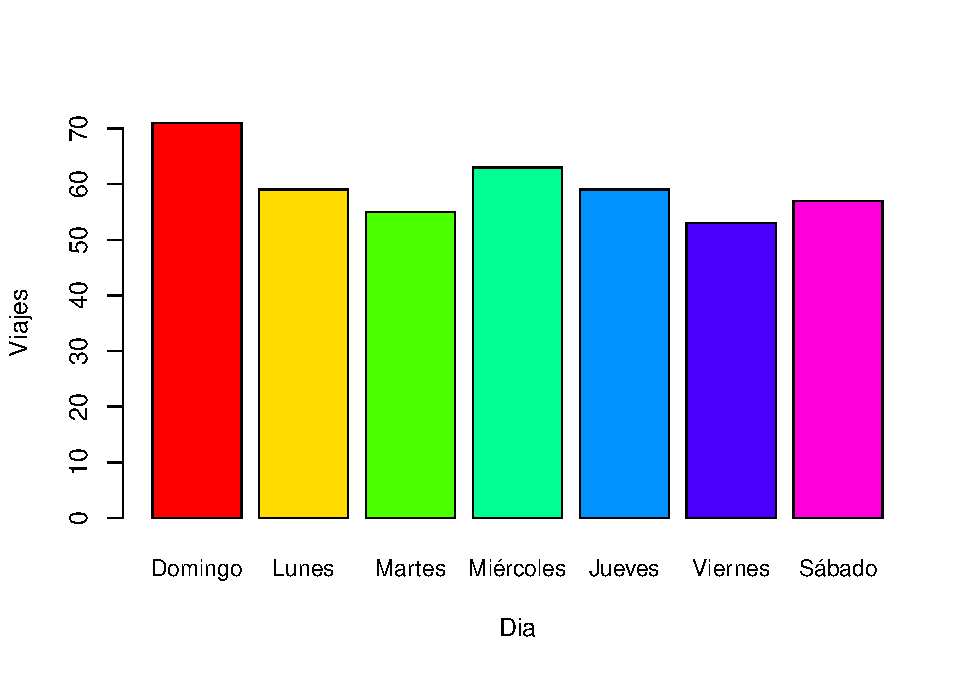
\includegraphics{notebook_files/figure-latex/unnamed-chunk-4-1.pdf}

Viajes por Sexo cada Dia

\begin{Shaded}
\begin{Highlighting}[]
\NormalTok{viajes\_sexo\_semana }\OtherTok{=} \FunctionTok{table}\NormalTok{(usuarios\_recorridos}\SpecialCharTok{$}\NormalTok{genero\_usuario, usuarios\_recorridos}\SpecialCharTok{$}\NormalTok{dia)}
\FunctionTok{barplot}\NormalTok{(viajes\_sexo\_semana, }\AttributeTok{xlab =} \StringTok{"Dia"}\NormalTok{, }\AttributeTok{ylab =} \StringTok{"Viajes"}\NormalTok{, }\AttributeTok{names =} \FunctionTok{levels}\NormalTok{(dias), }\AttributeTok{col =} \FunctionTok{c}\NormalTok{(}\StringTok{"\#FF8989"}\NormalTok{, }\StringTok{"\#A6F6F1"}\NormalTok{, }\StringTok{"\#CEFA8A"}\NormalTok{), }\AttributeTok{beside =} \ConstantTok{TRUE}\NormalTok{, }\AttributeTok{cex.names =} \FloatTok{0.9}\NormalTok{, }\AttributeTok{ylim =} \FunctionTok{c}\NormalTok{(}\DecValTok{0}\NormalTok{,}\DecValTok{40}\NormalTok{))}
\FunctionTok{legend}\NormalTok{(}\StringTok{"topright"}\NormalTok{, }\AttributeTok{legend =} \FunctionTok{c}\NormalTok{(}\StringTok{"Mujeres"}\NormalTok{, }\StringTok{"Hombres"}\NormalTok{, }\StringTok{"Otros"}\NormalTok{), }\AttributeTok{fill =} \FunctionTok{c}\NormalTok{(}\StringTok{"\#FF8989"}\NormalTok{, }\StringTok{"\#A6F6F1"}\NormalTok{, }\StringTok{"\#CEFA8A"}\NormalTok{))}
\end{Highlighting}
\end{Shaded}

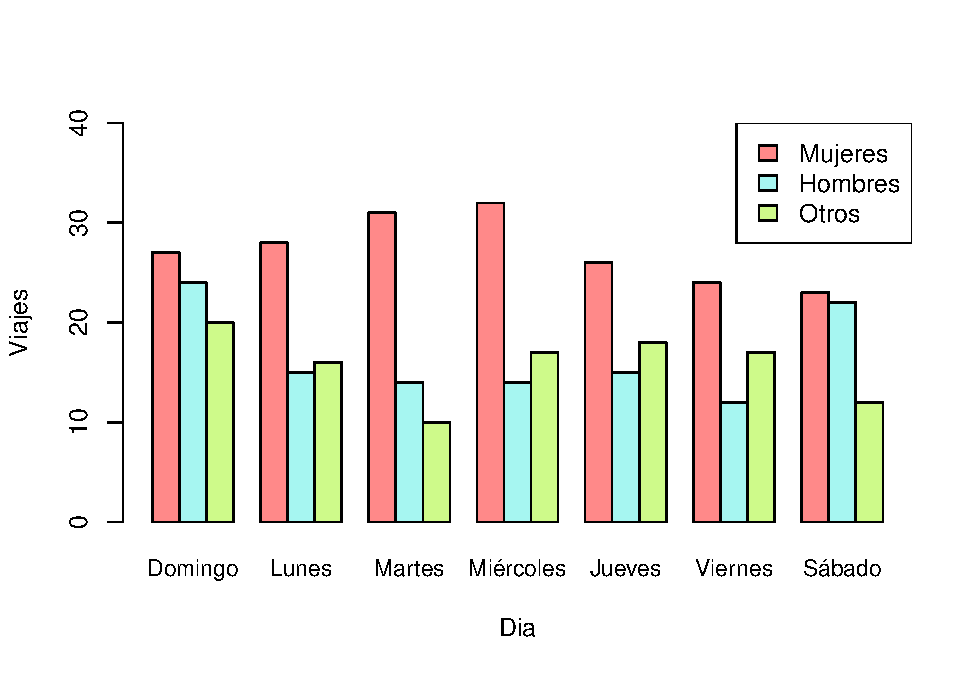
\includegraphics{notebook_files/figure-latex/unnamed-chunk-5-1.pdf}

Usuarios por Sexo

\begin{Shaded}
\begin{Highlighting}[]
\NormalTok{usuarios\_generos }\OtherTok{=} \FunctionTok{table}\NormalTok{(usuarios}\SpecialCharTok{$}\NormalTok{genero\_usuario)}
\NormalTok{porcentajes\_generos }\OtherTok{=}\NormalTok{ usuarios\_generos}
\NormalTok{porcentajes\_generos }\OtherTok{=} \FunctionTok{paste}\NormalTok{(}\FunctionTok{c}\NormalTok{(}\StringTok{"Mujeres"}\NormalTok{, }\StringTok{"Hombres"}\NormalTok{, }\StringTok{"Otros"}\NormalTok{), porcentajes\_generos)}
\NormalTok{porcentajes\_generos }\OtherTok{=} \FunctionTok{paste}\NormalTok{(porcentajes\_generos, }\StringTok{"\%"}\NormalTok{, }\AttributeTok{sep =} \StringTok{""}\NormalTok{)}
\FunctionTok{pie}\NormalTok{(usuarios\_generos, }\AttributeTok{labels =}\NormalTok{ porcentajes\_generos, }\AttributeTok{col =} \FunctionTok{c}\NormalTok{(}\StringTok{"\#FF8989"}\NormalTok{, }\StringTok{"\#A6F6F1"}\NormalTok{, }\StringTok{"\#CEFA8A"}\NormalTok{))}
\end{Highlighting}
\end{Shaded}

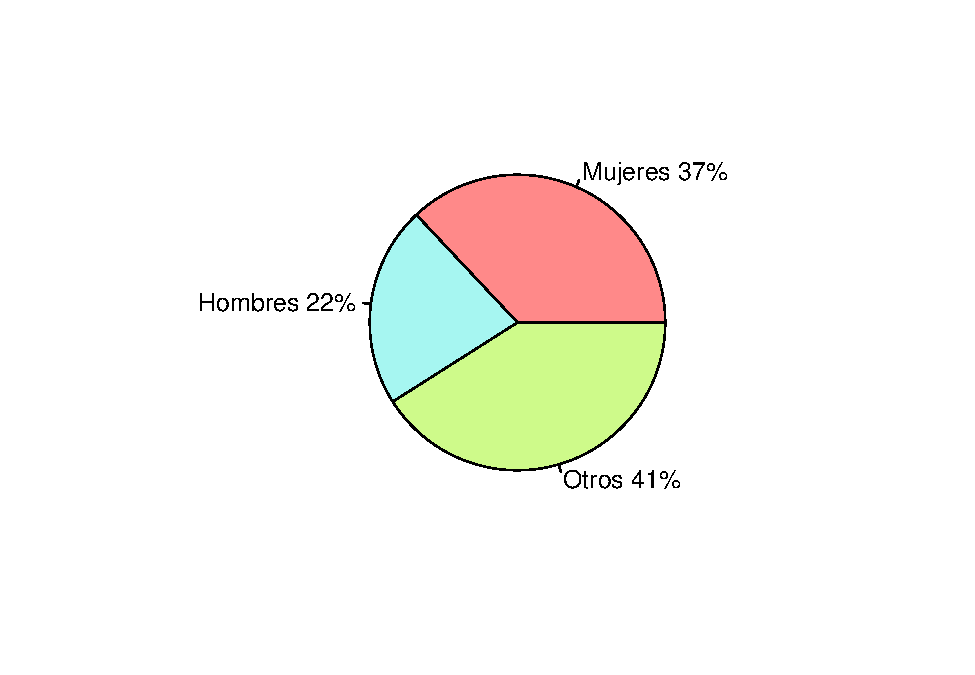
\includegraphics{notebook_files/figure-latex/unnamed-chunk-6-1.pdf}

Viajes Sexos

\begin{Shaded}
\begin{Highlighting}[]
\NormalTok{viajes\_sexo }\OtherTok{=} \FunctionTok{table}\NormalTok{(usuarios\_recorridos}\SpecialCharTok{$}\NormalTok{genero\_usuario)}
\NormalTok{porcentajes\_viajes\_sexo }\OtherTok{=} \FunctionTok{round}\NormalTok{((viajes\_sexo }\SpecialCharTok{*} \DecValTok{100}\NormalTok{)}\SpecialCharTok{/}\DecValTok{417}\NormalTok{)}
\NormalTok{porcentajes\_viajes\_sexo }\OtherTok{=} \FunctionTok{paste}\NormalTok{(}\FunctionTok{c}\NormalTok{(}\StringTok{"Mujeres"}\NormalTok{, }\StringTok{"Hombres"}\NormalTok{, }\StringTok{"Otros"}\NormalTok{), porcentajes\_viajes\_sexo)}
\NormalTok{porcentajes\_viajes\_sexo }\OtherTok{=} \FunctionTok{paste}\NormalTok{(porcentajes\_viajes\_sexo, }\StringTok{"\%"}\NormalTok{, }\AttributeTok{sep =} \StringTok{""}\NormalTok{)}
\FunctionTok{pie}\NormalTok{(viajes\_sexo, }\AttributeTok{labels =}\NormalTok{ porcentajes\_viajes\_sexo, }\AttributeTok{col =} \FunctionTok{c}\NormalTok{(}\StringTok{"\#FF8989"}\NormalTok{, }\StringTok{"\#A6F6F1"}\NormalTok{, }\StringTok{"\#CEFA8A"}\NormalTok{))}
\end{Highlighting}
\end{Shaded}

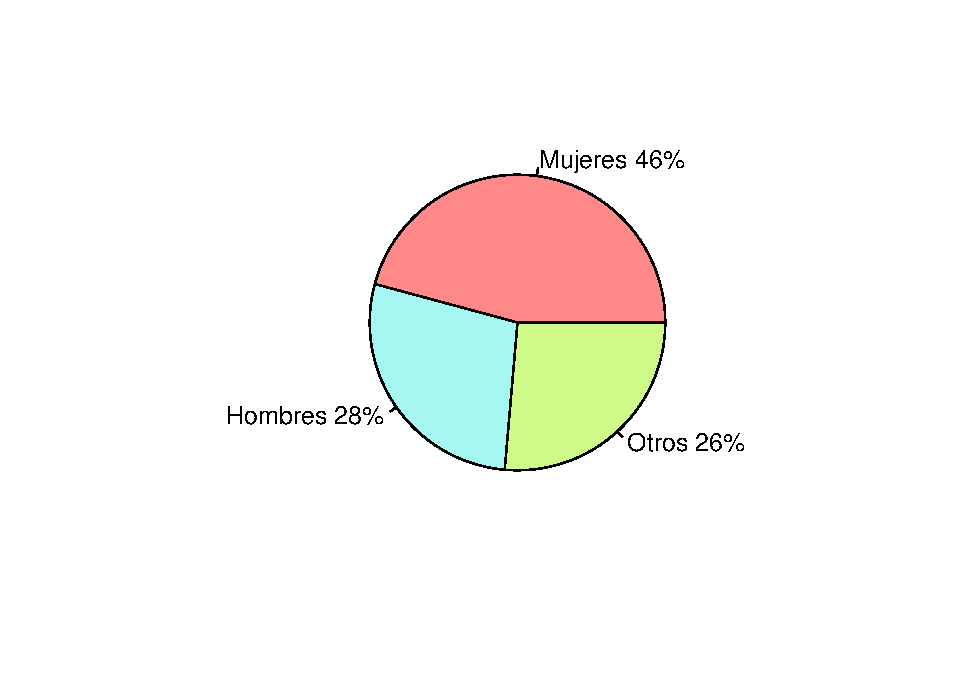
\includegraphics{notebook_files/figure-latex/unnamed-chunk-7-1.pdf}

Usuarios por Edad (tallo y hoja, e histograma)

\begin{Shaded}
\begin{Highlighting}[]
\FunctionTok{stem}\NormalTok{(usuarios}\SpecialCharTok{$}\NormalTok{edad\_usuario, }\AttributeTok{atom =} \DecValTok{10}\NormalTok{)}
\end{Highlighting}
\end{Shaded}

\begin{verbatim}
## 
##   The decimal point is 1 digit(s) to the right of the |
## 
##   1 | 888999
##   2 | 00000111222223333333555566777777778899999
##   3 | 0000011111112222334455566777788
##   4 | 00113445568
##   5 | 01111124
##   6 | 035
\end{verbatim}

\begin{Shaded}
\begin{Highlighting}[]
\FunctionTok{hist}\NormalTok{(usuarios}\SpecialCharTok{$}\NormalTok{edad\_usuario, }\AttributeTok{main =} \StringTok{""}\NormalTok{, }\AttributeTok{xlab =} \StringTok{"Edades"}\NormalTok{, }\AttributeTok{ylab =} \StringTok{"Cantidad"}\NormalTok{, }\AttributeTok{col =} \StringTok{"purple"}\NormalTok{, }\AttributeTok{ylim =} \FunctionTok{c}\NormalTok{(}\DecValTok{0}\NormalTok{, }\DecValTok{25}\NormalTok{), }\AttributeTok{xaxp =} \FunctionTok{c}\NormalTok{(}\DecValTok{10}\NormalTok{, }\DecValTok{65}\NormalTok{, }\DecValTok{11}\NormalTok{))}
\end{Highlighting}
\end{Shaded}

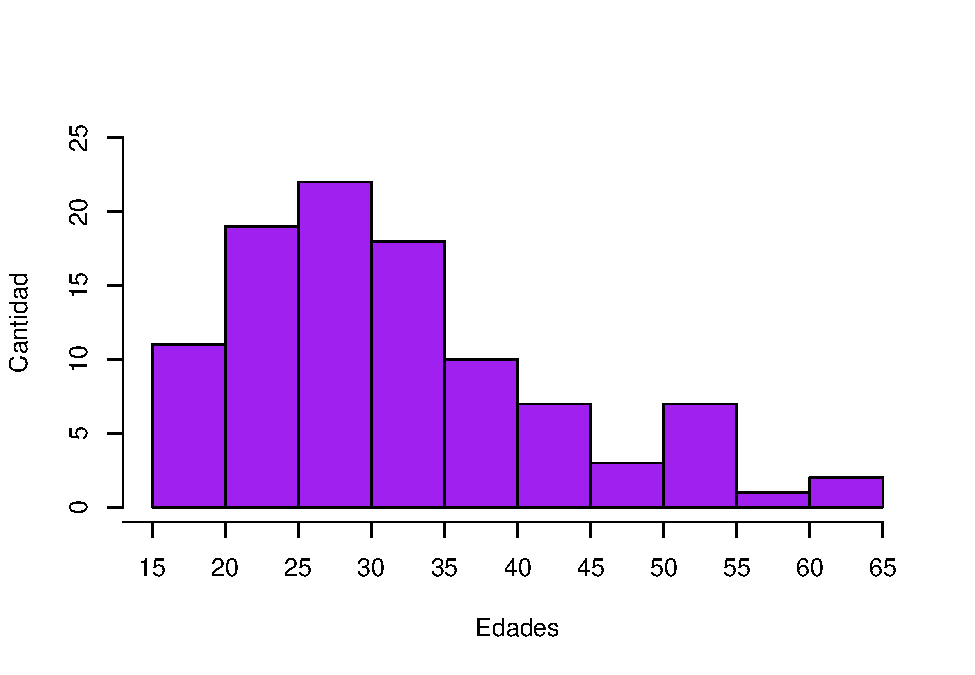
\includegraphics{notebook_files/figure-latex/unnamed-chunk-8-1.pdf}

Viajes Edades

\begin{Shaded}
\begin{Highlighting}[]
\FunctionTok{hist}\NormalTok{(usuarios\_recorridos}\SpecialCharTok{$}\NormalTok{edad\_usuario, }\AttributeTok{main =} \StringTok{""}\NormalTok{, }\AttributeTok{xlab =} \StringTok{"Edades"}\NormalTok{, }\AttributeTok{ylab =} \StringTok{"Cantidad"}\NormalTok{, }\AttributeTok{col =} \StringTok{"purple"}\NormalTok{, }\AttributeTok{ylim =} \FunctionTok{c}\NormalTok{(}\DecValTok{0}\NormalTok{, }\DecValTok{140}\NormalTok{), }\AttributeTok{xaxp =} \FunctionTok{c}\NormalTok{(}\DecValTok{10}\NormalTok{, }\DecValTok{65}\NormalTok{, }\DecValTok{11}\NormalTok{))}
\end{Highlighting}
\end{Shaded}

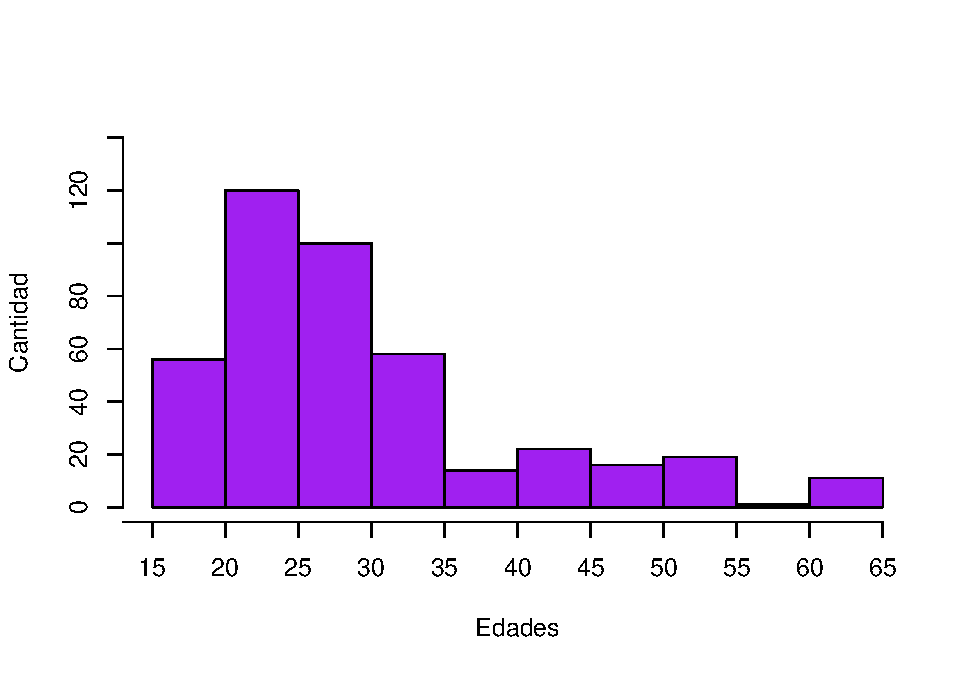
\includegraphics{notebook_files/figure-latex/unnamed-chunk-9-1.pdf}

Tabla viajes Edades

\begin{Shaded}
\begin{Highlighting}[]
\NormalTok{intervalos\_edades }\OtherTok{=} \FunctionTok{cut}\NormalTok{(usuarios\_recorridos}\SpecialCharTok{$}\NormalTok{edad\_usuario, }\AttributeTok{breaks =} \FunctionTok{c}\NormalTok{(}\DecValTok{15}\NormalTok{, }\DecValTok{20}\NormalTok{, }\DecValTok{25}\NormalTok{, }\DecValTok{30}\NormalTok{, }\DecValTok{35}\NormalTok{, }\DecValTok{40}\NormalTok{, }\DecValTok{45}\NormalTok{, }\DecValTok{50}\NormalTok{, }\DecValTok{55}\NormalTok{, }\DecValTok{60}\NormalTok{, }\DecValTok{65}\NormalTok{))}
\NormalTok{frecuencia\_absoluta }\OtherTok{=} \FunctionTok{table}\NormalTok{(intervalos\_edades)}
\NormalTok{frecuencia\_relativa }\OtherTok{=} \FunctionTok{prop.table}\NormalTok{(frecuencia\_absoluta)}
\NormalTok{porcentaje }\OtherTok{=}\NormalTok{ frecuencia\_relativa }\SpecialCharTok{*} \DecValTok{100}
\NormalTok{frecuencia\_absoluta\_acumulada }\OtherTok{=} \FunctionTok{cumsum}\NormalTok{(frecuencia\_absoluta)}
\NormalTok{frecuencia\_relativa\_acumulada }\OtherTok{=} \FunctionTok{cumsum}\NormalTok{(frecuencia\_relativa)}
\NormalTok{porcentaje\_acumulado }\OtherTok{=} \FunctionTok{cumsum}\NormalTok{(porcentaje)}
\NormalTok{tabla\_edad }\OtherTok{=} \FunctionTok{cbind}\NormalTok{(frecuencia\_absoluta, frecuencia\_relativa, porcentaje, frecuencia\_absoluta\_acumulada, frecuencia\_relativa\_acumulada, porcentaje\_acumulado)}
\FunctionTok{kable}\NormalTok{(tabla\_edad, }\AttributeTok{caption =} \StringTok{"Viajes por Franjas Etarias"}\NormalTok{, }\AttributeTok{col.names =} \FunctionTok{c}\NormalTok{(}\StringTok{"Frecuencia Absoluta"}\NormalTok{, }\StringTok{"Frecuencia Relativa"}\NormalTok{, }\StringTok{"Porcentaje"}\NormalTok{, }\StringTok{"Frec abs acumulada"}\NormalTok{, }\StringTok{"Frec rel acumulada"}\NormalTok{, }\StringTok{"Porc acumulado"}\NormalTok{), }\AttributeTok{digits =} \DecValTok{2}\NormalTok{, }\AttributeTok{align =} \StringTok{"cccccc"}\NormalTok{)}
\end{Highlighting}
\end{Shaded}

\begin{longtable}[]{@{}
  >{\raggedright\arraybackslash}p{(\columnwidth - 12\tabcolsep) * \real{0.07}}
  >{\centering\arraybackslash}p{(\columnwidth - 12\tabcolsep) * \real{0.18}}
  >{\centering\arraybackslash}p{(\columnwidth - 12\tabcolsep) * \real{0.18}}
  >{\centering\arraybackslash}p{(\columnwidth - 12\tabcolsep) * \real{0.10}}
  >{\centering\arraybackslash}p{(\columnwidth - 12\tabcolsep) * \real{0.17}}
  >{\centering\arraybackslash}p{(\columnwidth - 12\tabcolsep) * \real{0.17}}
  >{\centering\arraybackslash}p{(\columnwidth - 12\tabcolsep) * \real{0.14}}@{}}
\caption{Viajes por Franjas Etarias}\tabularnewline
\toprule
& Frecuencia Absoluta & Frecuencia Relativa & Porcentaje & Frec abs
acumulada & Frec rel acumulada & Porc acumulado \\
\midrule
\endfirsthead
\toprule
& Frecuencia Absoluta & Frecuencia Relativa & Porcentaje & Frec abs
acumulada & Frec rel acumulada & Porc acumulado \\
\midrule
\endhead
(15,20{]} & 56 & 0.13 & 13.43 & 56 & 0.13 & 13.43 \\
(20,25{]} & 120 & 0.29 & 28.78 & 176 & 0.42 & 42.21 \\
(25,30{]} & 100 & 0.24 & 23.98 & 276 & 0.66 & 66.19 \\
(30,35{]} & 58 & 0.14 & 13.91 & 334 & 0.80 & 80.10 \\
(35,40{]} & 14 & 0.03 & 3.36 & 348 & 0.83 & 83.45 \\
(40,45{]} & 22 & 0.05 & 5.28 & 370 & 0.89 & 88.73 \\
(45,50{]} & 16 & 0.04 & 3.84 & 386 & 0.93 & 92.57 \\
(50,55{]} & 19 & 0.05 & 4.56 & 405 & 0.97 & 97.12 \\
(55,60{]} & 1 & 0.00 & 0.24 & 406 & 0.97 & 97.36 \\
(60,65{]} & 11 & 0.03 & 2.64 & 417 & 1.00 & 100.00 \\
\bottomrule
\end{longtable}

Boxplot Tiempo de uso

\begin{Shaded}
\begin{Highlighting}[]
\FunctionTok{boxplot}\NormalTok{(recorridos}\SpecialCharTok{$}\NormalTok{duracion\_recorrido, }\AttributeTok{horizontal =} \ConstantTok{TRUE}\NormalTok{, }\AttributeTok{xlab =} \StringTok{"Duracion de viaje (en segundos)"}\NormalTok{, }\AttributeTok{boxfill=}\StringTok{"lightblue"}\NormalTok{, }\AttributeTok{outline =} \ConstantTok{FALSE}\NormalTok{)}
\end{Highlighting}
\end{Shaded}

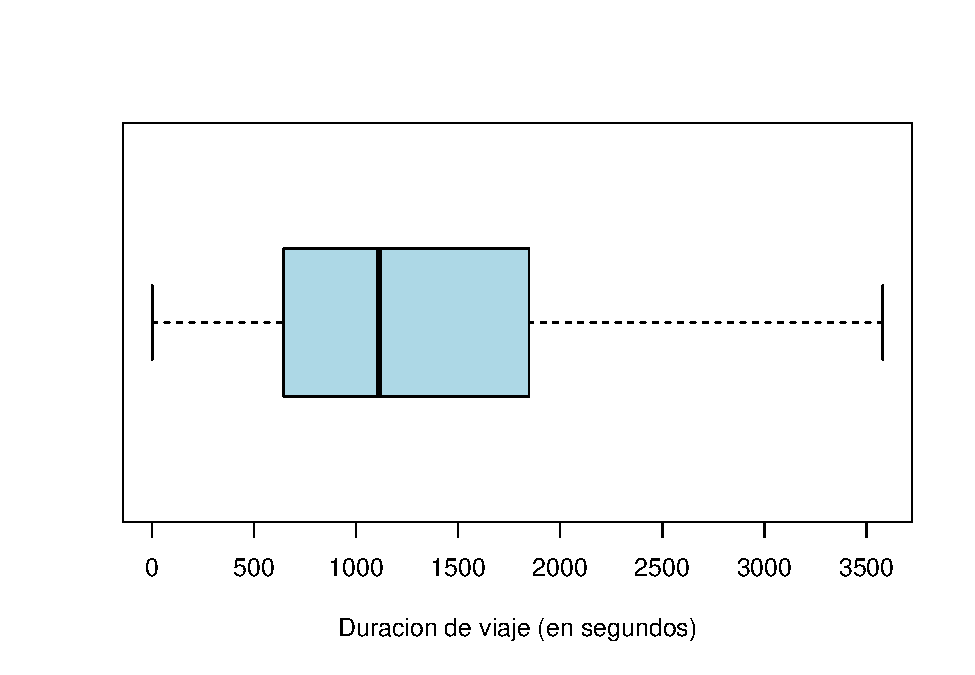
\includegraphics{notebook_files/figure-latex/unnamed-chunk-11-1.pdf}

\begin{Shaded}
\begin{Highlighting}[]
\FunctionTok{boxplot}\NormalTok{(recorridos}\SpecialCharTok{$}\NormalTok{duracion\_recorrido, }\AttributeTok{horizontal =} \ConstantTok{TRUE}\NormalTok{, }\AttributeTok{xlab =} \StringTok{"Duracion de viaje (en segundos)"}\NormalTok{, }\AttributeTok{boxfill=}\StringTok{"lightblue"}\NormalTok{)}
\end{Highlighting}
\end{Shaded}

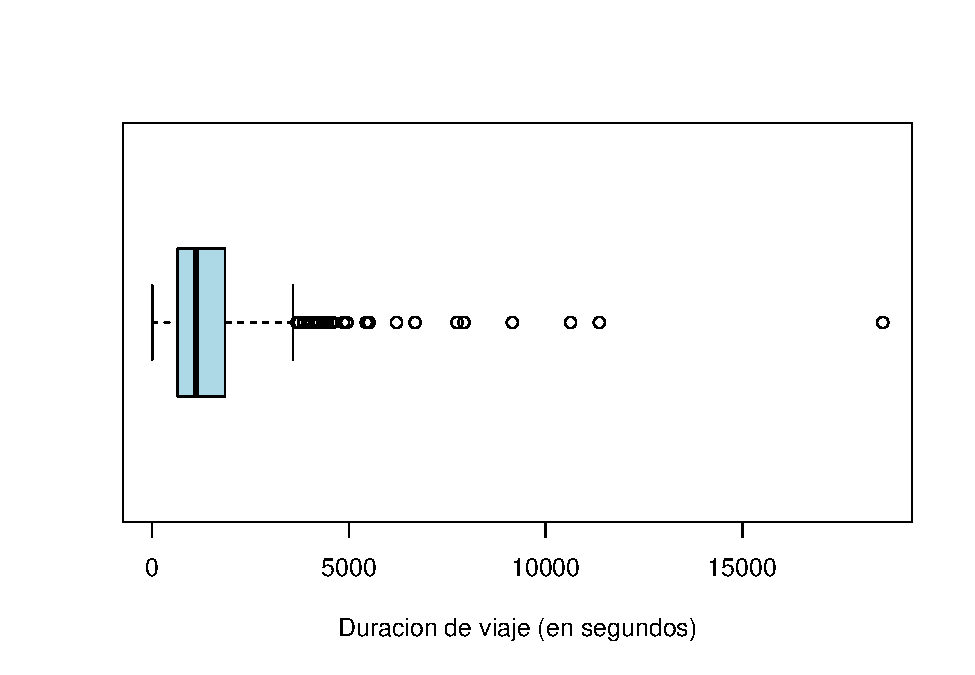
\includegraphics{notebook_files/figure-latex/unnamed-chunk-11-2.pdf}

\begin{Shaded}
\begin{Highlighting}[]
\NormalTok{intervalos\_horas }\OtherTok{=} \FunctionTok{cut}\NormalTok{(recorridos}\SpecialCharTok{$}\NormalTok{duracion\_recorrido, }\AttributeTok{breaks =} \FunctionTok{c}\NormalTok{(}\DecValTok{0}\NormalTok{, }\DecValTok{1800}\NormalTok{, }\DecValTok{3600}\NormalTok{, }\DecValTok{5400}\NormalTok{, }\DecValTok{19800}\NormalTok{), }\AttributeTok{dig.lab =} \DecValTok{10}\NormalTok{)}
\NormalTok{frecuencia\_absoluta }\OtherTok{=} \FunctionTok{table}\NormalTok{(intervalos\_horas)}
\NormalTok{frecuencia\_relativa }\OtherTok{=} \FunctionTok{prop.table}\NormalTok{(frecuencia\_absoluta)}
\NormalTok{porcentaje }\OtherTok{=}\NormalTok{ frecuencia\_relativa }\SpecialCharTok{*} \DecValTok{100}
\NormalTok{frecuencia\_absoluta\_acumulada }\OtherTok{=} \FunctionTok{cumsum}\NormalTok{(frecuencia\_absoluta)}
\NormalTok{frecuencia\_relativa\_acumulada }\OtherTok{=} \FunctionTok{cumsum}\NormalTok{(frecuencia\_relativa)}
\NormalTok{porcentaje\_acumulado }\OtherTok{=} \FunctionTok{cumsum}\NormalTok{(porcentaje)}
\NormalTok{tabla\_duracion\_recorridos }\OtherTok{=} \FunctionTok{cbind}\NormalTok{(frecuencia\_absoluta, frecuencia\_relativa, porcentaje, frecuencia\_absoluta\_acumulada, frecuencia\_relativa\_acumulada, porcentaje\_acumulado)}
\FunctionTok{kable}\NormalTok{(tabla\_duracion\_recorridos, }\AttributeTok{caption =} \StringTok{"Duraciones de recorridos"}\NormalTok{, }\AttributeTok{col.names =} \FunctionTok{c}\NormalTok{(}\StringTok{"Frecuencia Absoluta"}\NormalTok{, }\StringTok{"Frecuencia Relativa"}\NormalTok{, }\StringTok{"Porcentaje"}\NormalTok{, }\StringTok{"Frec abs acumulada"}\NormalTok{, }\StringTok{"Frec rel acumulada"}\NormalTok{, }\StringTok{"Porc acumulado"}\NormalTok{), }\AttributeTok{digits =} \DecValTok{2}\NormalTok{, }\AttributeTok{align =} \StringTok{"cccccc"}\NormalTok{)}
\end{Highlighting}
\end{Shaded}

\begin{longtable}[]{@{}
  >{\raggedright\arraybackslash}p{(\columnwidth - 12\tabcolsep) * \real{0.11}}
  >{\centering\arraybackslash}p{(\columnwidth - 12\tabcolsep) * \real{0.17}}
  >{\centering\arraybackslash}p{(\columnwidth - 12\tabcolsep) * \real{0.17}}
  >{\centering\arraybackslash}p{(\columnwidth - 12\tabcolsep) * \real{0.10}}
  >{\centering\arraybackslash}p{(\columnwidth - 12\tabcolsep) * \real{0.16}}
  >{\centering\arraybackslash}p{(\columnwidth - 12\tabcolsep) * \real{0.16}}
  >{\centering\arraybackslash}p{(\columnwidth - 12\tabcolsep) * \real{0.13}}@{}}
\caption{Duraciones de recorridos}\tabularnewline
\toprule
& Frecuencia Absoluta & Frecuencia Relativa & Porcentaje & Frec abs
acumulada & Frec rel acumulada & Porc acumulado \\
\midrule
\endfirsthead
\toprule
& Frecuencia Absoluta & Frecuencia Relativa & Porcentaje & Frec abs
acumulada & Frec rel acumulada & Porc acumulado \\
\midrule
\endhead
(0,1800{]} & 308 & 0.74 & 73.86 & 308 & 0.74 & 73.86 \\
(1800,3600{]} & 81 & 0.19 & 19.42 & 389 & 0.93 & 93.29 \\
(3600,5400{]} & 18 & 0.04 & 4.32 & 407 & 0.98 & 97.60 \\
(5400,19800{]} & 10 & 0.02 & 2.40 & 417 & 1.00 & 100.00 \\
\bottomrule
\end{longtable}

Boxplot Distancia

\begin{Shaded}
\begin{Highlighting}[]
\FunctionTok{boxplot}\NormalTok{(recorridos}\SpecialCharTok{$}\NormalTok{distancia, }\AttributeTok{horizontal =} \ConstantTok{TRUE}\NormalTok{, }\AttributeTok{xlab =} \StringTok{"Distancia (en metros)"}\NormalTok{, }\AttributeTok{boxfill=}\StringTok{"lightblue"}\NormalTok{)}
\end{Highlighting}
\end{Shaded}

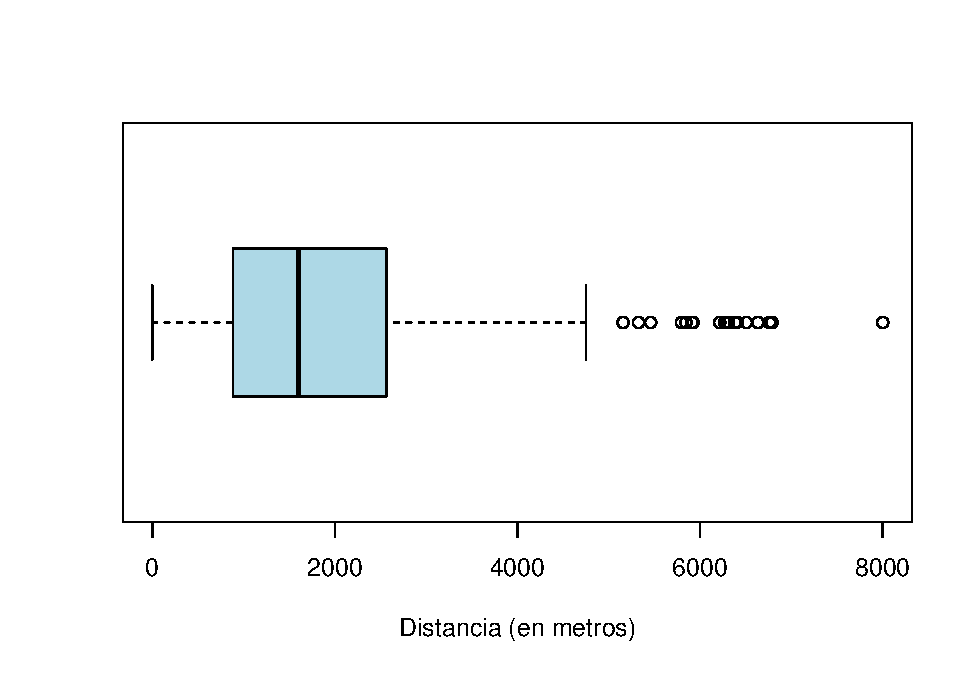
\includegraphics{notebook_files/figure-latex/unnamed-chunk-12-1.pdf}

\begin{Shaded}
\begin{Highlighting}[]
\FunctionTok{plot}\NormalTok{(recorridos}\SpecialCharTok{$}\NormalTok{duracion\_recorrido}\SpecialCharTok{\textasciitilde{}}\NormalTok{recorridos}\SpecialCharTok{$}\NormalTok{distancia,}\AttributeTok{ylab =} \StringTok{"Duración"}\NormalTok{,}\AttributeTok{xlab =} \StringTok{"Distancia"}\NormalTok{)}
\end{Highlighting}
\end{Shaded}

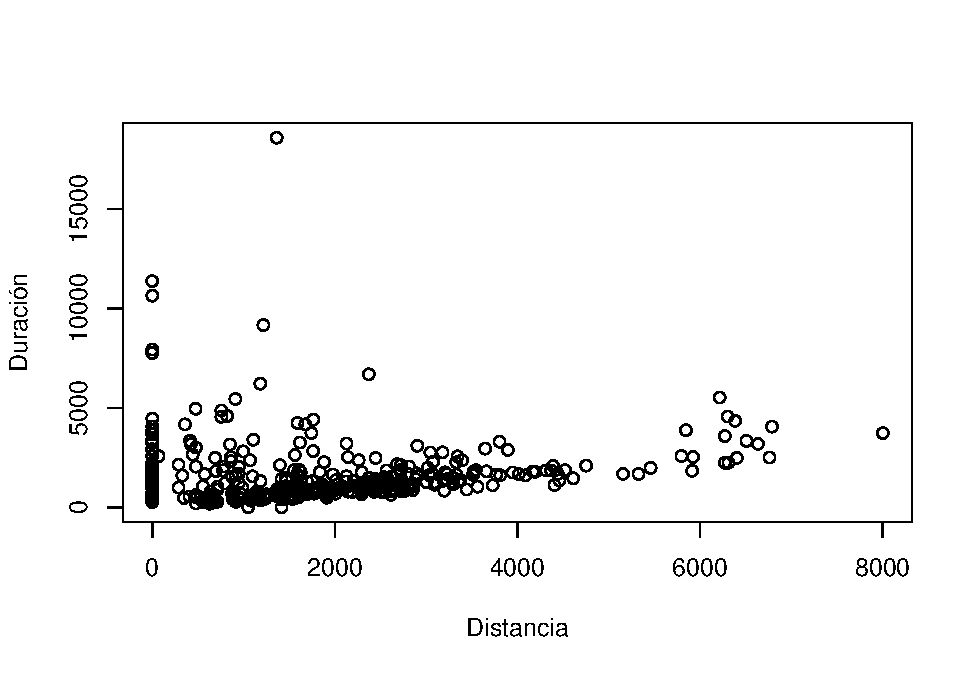
\includegraphics{notebook_files/figure-latex/unnamed-chunk-12-2.pdf}

Boxplot Distancia

\begin{Shaded}
\begin{Highlighting}[]
\FunctionTok{boxplot}\NormalTok{(recorridos}\SpecialCharTok{$}\NormalTok{distancia, }\AttributeTok{horizontal =} \ConstantTok{TRUE}\NormalTok{, }\AttributeTok{xlab =} \StringTok{"Distancia (en metros)"}\NormalTok{, }\AttributeTok{boxfill=}\StringTok{"lightblue"}\NormalTok{)}
\end{Highlighting}
\end{Shaded}

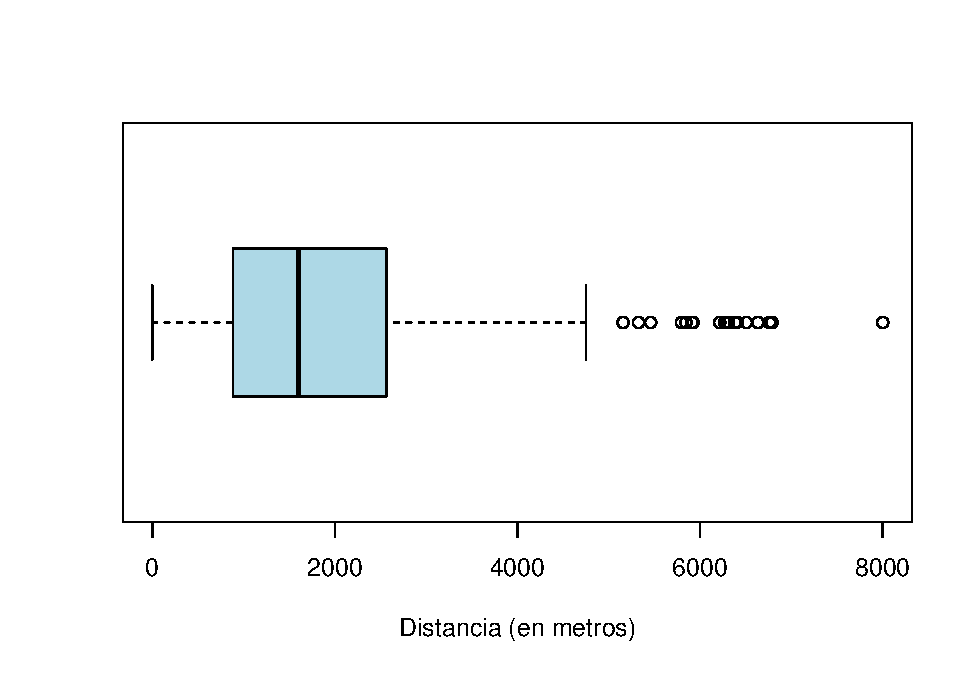
\includegraphics{notebook_files/figure-latex/unnamed-chunk-13-1.pdf}

\begin{Shaded}
\begin{Highlighting}[]
\FunctionTok{plot}\NormalTok{(recorridos}\SpecialCharTok{$}\NormalTok{duracion\_recorrido}\SpecialCharTok{\textasciitilde{}}\NormalTok{recorridos}\SpecialCharTok{$}\NormalTok{distancia,}\AttributeTok{ylab =} \StringTok{"Duración"}\NormalTok{,}\AttributeTok{xlab =} \StringTok{"Distancia"}\NormalTok{)}
\end{Highlighting}
\end{Shaded}

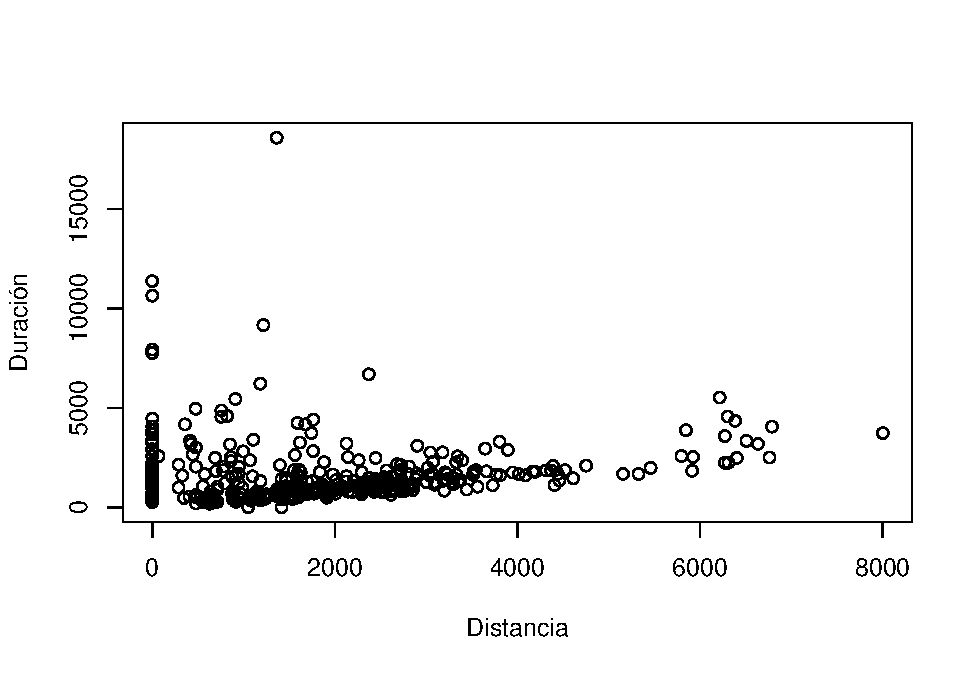
\includegraphics{notebook_files/figure-latex/unnamed-chunk-13-2.pdf}

Grafico de putos

\begin{Shaded}
\begin{Highlighting}[]
\NormalTok{usuarios\_factor }\OtherTok{=} \FunctionTok{as.factor}\NormalTok{(recorridos}\SpecialCharTok{$}\NormalTok{id\_usuario)}
\NormalTok{usuarios\_factor }\OtherTok{=} \FunctionTok{table}\NormalTok{(usuarios\_factor)}
\NormalTok{dir\_data }\OtherTok{=} \FunctionTok{as.data.frame}\NormalTok{(usuarios\_factor)}
\FunctionTok{stripchart}\NormalTok{(dir\_data}\SpecialCharTok{$}\NormalTok{Freq,}\AttributeTok{method=}\StringTok{"stack"}\NormalTok{,}\AttributeTok{xlab=}\StringTok{"Viajes"}\NormalTok{,}\AttributeTok{offset=}\FloatTok{0.5}\NormalTok{,}\AttributeTok{at=}\FloatTok{0.01}\NormalTok{,}\AttributeTok{pch=}\DecValTok{19}\NormalTok{)}
\end{Highlighting}
\end{Shaded}

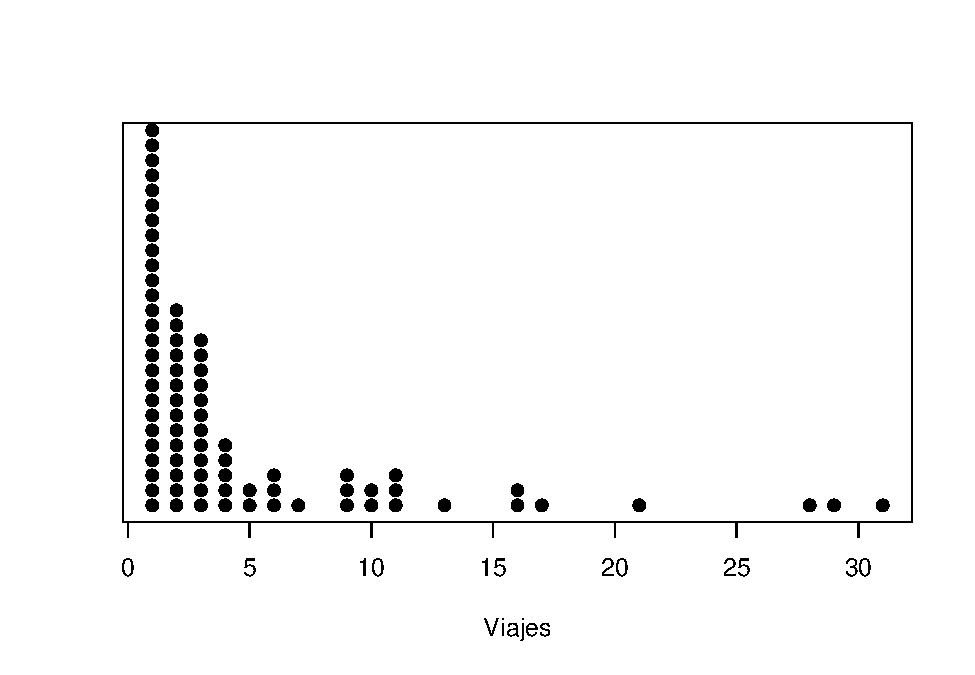
\includegraphics{notebook_files/figure-latex/unnamed-chunk-14-1.pdf}

\end{document}
